\chapter{Implementierung}
\label{cha:implementation}

Die Implementierung des Compilers ist in zwei Teile aufgeteilt: Frontend und Backend. Die Kommunikation zwischen den beiden Teilen erfolgt mithilfe eines abstrakten Syntaxbaums (AST - \textit{abstract syntax tree}), welchen das Frontend erzeugt. Dieses Kapitel geht  auf die Architektur und Implementierung dieser Teile ein.~\autoref{fig:compiler-architecture} zeigt die Archtektur des \toya Compilers. Auf die genauere Implementierung der verschiedenen Schritte des Compilers geht dieses Kapitel ein.

Die Implementierung erfolgt in Kotlin, was das Einbinden von bereits existierende Bibliotheken des JVM Ökosystems problemlos ermöglicht. Konkret geht es dabei um ANTLR und ObjectWeb ASM, welche wichtige Rollen im Compiler übernehmen. Die Möglichkeit, Summentypen in Form von \textit{sealed} Schnittstellen und Klassen implementieren zu können, erleichert die Abarbeitung des ASTs wesentlich.

\begin{figure}[h]
    \caption{Compiler-Architektur}
    \centering
    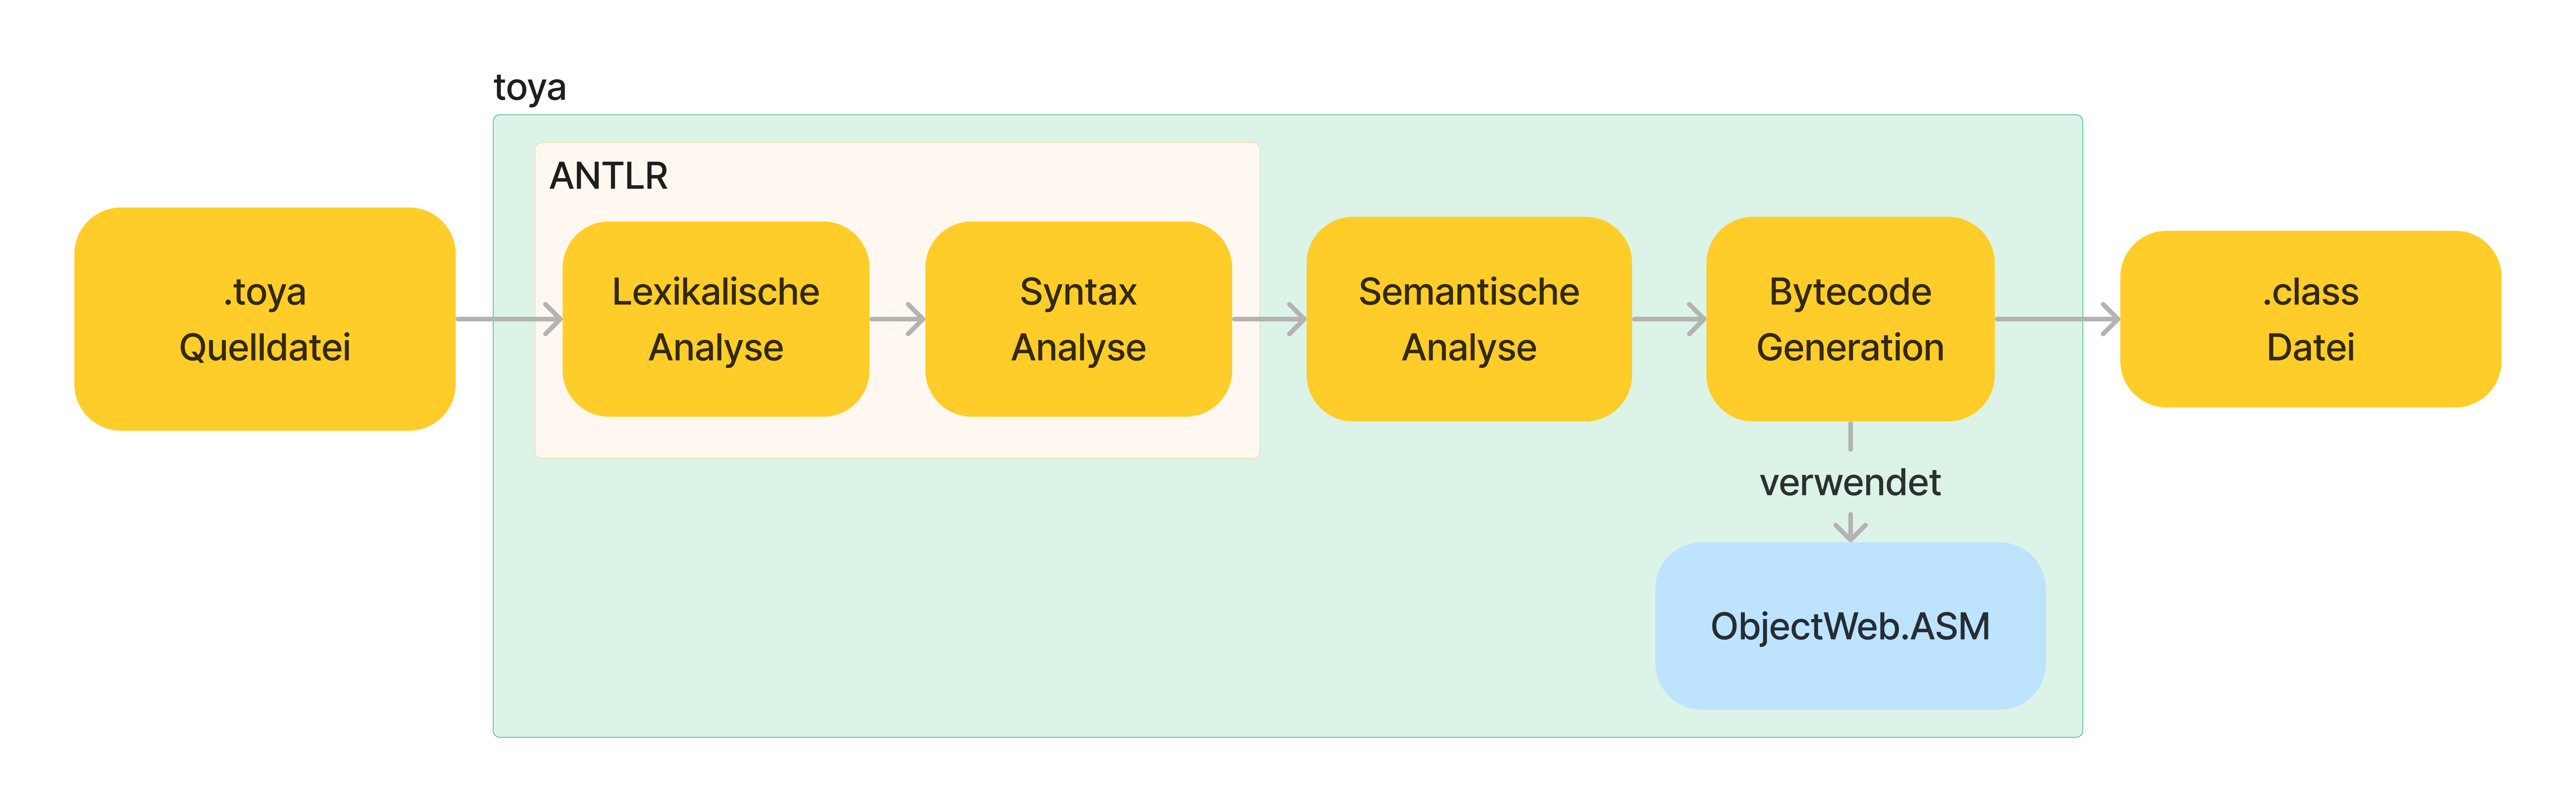
\includegraphics[width=\textwidth]{Compiler.Architecture}
    \label{fig:compiler-architecture}
\end{figure}

\section{Frontend}

Im Frontend erfolgt die lexikalische, syntaktische und teilweise die semantische Analyse. Die lexikalische Analyse zerlegt anhand der bereitgestellten Grammatik den Quellcode in \token. Anhand dieser \token erstellt die syntaktische Analyse den Syntaxbaum, welcher als Basis für den abstrakten Syntaxbaum dient.

\subsection{Grammatik}

Als Ausgangspunkt des Frontends dient die Grammatik, anhand welcher ANTLR die lexikalische und syntaktische Analyse implementiert. Diese Grammatik definiert die Compiler-Bauer:in in einer \texttt{g4}-Datei. Leerzeichen haben keine semantische Relevanz, weshalb \toya diese in der syntaktischen Analyse überspringt. Als \token definiert \toya folgende Zeichen:

\begin{itemize}
    \item Die Schlüsselwörter \texttt{match}, \texttt{for}, \texttt{for}, \texttt{if}, \texttt{else}, \texttt{var}, \texttt{true}, \texttt{false} und \texttt{null}
    \item Die Infix-Operatoren \texttt{>}, \texttt{>=}, \texttt{<}, \texttt{<=}, \texttt{==}, \texttt{!=}, \texttt{\&\&}, \texttt{||} und der Präfix-Operator \texttt{!}
    \item Die arithmetischen Operatoren \texttt{+}, \texttt{-}, \texttt{*} und \texttt{/}
\end{itemize}

Beim Versuch, ein Schlüsselwort als Variablenname zu Verwenden tritt der Ausnahmezustand \texttt{VariableNameIsKeywordException} ein. 

\subsection{Abarbeitung des Syntaxbaum}

Wie bereits in \nameref{cha:antlr} erläutert, bietet ANTLR die Entwurfsmuster \visitor und \listener an, um den Syntaxbaum zu traversieren. \Toya verwendet das \visitor-Muster aufgrund des Umfangs des zu traversierenden Syntaxbaums. Das Resultat des \visitors ist ein AST mit dem Wurzelelement \texttt{Compilation}. Diese Klasse speichert die Funktionssignaturen, globale Variablen und ein globales \scope, welches sich über das ganze Programm erstreckt. Alle weiteren \texttt{Scopes} nehmen dieses globale \scope als Grundlage. 

Die wichtigste Methode des \visitor, welche die Abarbeitung des Syntaxbaums überhaupt ermöglicht ist die \texttt{accept} Methode. Diese Methode benötigt als Parameter einen \visitor vom generischen Typ \texttt{ParseTreeVisitor}. \Toya implementiert folgende \visitor:

\begin{itemize}
    \item CompilationVisitor
    \item StatementVisitor
    \item BranchVisitor
    \item CompositeVisitor
    \item ExpressionVisitor
    \item FunctionSignatureVisitor
    \item FunctionVisitor
\end{itemize}

Um das Traversieren der Knoten des Syntaxbaums zu ermöglichen, generiert ANTLR für alle Regeln der Grammatik-Definition Methoden im Format \texttt{visit<RuleName>(ctx: toyaParser.<RuleName>Context)}. Jede dieser Methoden liefert einen Wert vom generischen Typ des \texttt{toyaBaseVisitor} zurück.~\autoref{lst:impl_visitor} zeigt die \texttt{visit}-Funktion für Variablendeklarationen.

\begin{KotlinCode}[numbers=none, caption={\visitor-Funktion zum Erstellen eines \texttt{VariableDeclarationStatement}}, label=lst:impl_visitor]
class StatementVisitor(val scope: Scope) : toyaBaseVisitor<Statement>() {
    override fun visitVariableDeclaration(ctx: toyaParser.VariableDeclarationContext): Statement {
        val varName = ctx.name().text
        if(varName.isReservedKeyword()) throw VariableNameIsKeywordException(varName)
        val expression = ctx.expression().accept(ExpressionVisitor(scope))
        scope.addLocalVariable(LocalVariable(varName, expression.type))
        return VariableDeclarationStatement(varName, expression)
    }
    // Rest of class
}
\end{KotlinCode}

Zur Behandlung von Syntaxfehler bietet ANTLR die Klasse \texttt{BaseErrorListener} um der Benutzer:in relevante Informationen anzuzeigen. \Toya zeigt mithilfe dieser Klasse an, welche Anweisung in welcher Zeile und welches Zeichen die syntaktische Analyse verhindert.

\subsection{Typ-System}

Die Basis für das Typ-System in \toya ist die Schnittstelle \texttt{Type} und die davon abgeleitete Enum-Klasse \texttt{BasicType}, welche alle in \toya verfügbaren Typen umfasst. \Toya erlaubt keine explizite Definition des Typs einer Variable, weshalb der Typ immer vom Wert der Variable abzuleiten ist. Zum ermitteln des Typs kommt die Klasse \texttt{TypeResolver} zum Einsatz. Anhand von regulären Ausdrücken ermittelt dieser den Typ des Wert-Literals, wie in~\autoref{lst:impl_getvalue} zu sehen ist.

\begin{KotlinCode}[numbers=none, caption={Methode zur Ermittlung des Typs bei Wert-Literalen}, label={lst:getFromValue}, label=lst:impl_getvalue]
fun getFromValue(value: String?): Type {
    if (value.isNullOrEmpty()) return BasicType.VOID
    if (isBoolean(value)) return BasicType.BOOLEAN
    if (isDouble(value)) return BasicType.DOUBLE
    if (isInt(value)) return BasicType.INT
    if (isString(value)) return BasicType.STRING
    throw UnableToInferTypeException(value)
}
\end{KotlinCode}

Da nun die jeder Ausdruck Typinformationen besitzt, ermöglicht das die semantische Analyse von Ausdrücken. Die Erweiterungsfunktion \texttt{Type.checkTypeMatch} überprüft, ob beide Operanden vom selben Typ sind. Wenn nicht, kommt es zum Ausnahmezustand \texttt{BinaryOperationTypeMismatchException}. Die Implementierung für\break \texttt{Type.checkTypeMatch} ist in~\autoref{lst:impl_checktypematch} zu sehen.

\begin{KotlinCode}[numbers=none, caption={Methode zur Überprüfung, dass Operanden übereinstimmende Typen haben}, label=lst:impl_checktypematch]
fun Type.checkTypeMatch(rhs: Type) {
    if (this != rhs) throw BinaryOperationTypeMismatchException(this, rhs)
}    
\end{KotlinCode}

\subsection{Standardfunktionen}

Standardfunktionen sind Funktionen, welche jedem \toya-Programm ohne Weiteres zur Verfügung stehen. Standardfunktionen sind kein Bestandteil der lexikalischen Analyse. Die Funktion \texttt{visitFunctionCall} des \texttt{ExpressionVisitors} prüft mithilfe der Funktion \texttt{isStandardFunction}, ob es sich bei einer Funktion um eine Standardfunktion handelt. Ist dies der Fall, erzeugt der \visitor kein Objekt vom Typ \texttt{FunctionCall}, sondern ein Objekt, welches von \texttt{StandardFunction} erbt. Im Fall von \texttt{print} ist das zum Beispiel \texttt{PrintFunction}.

Standardmäßig bietet \toya die Standardfunktion \texttt{print} an, welche einen Aufruf der Java Funktion \texttt{System.out.println} durchführt. Die Architektur des \toya-Compilers ist darauf ausgelegt, weitere Standardfunktionen hinzufügen zu können. Besteht dieser Wunsch, sind an folgenden Stellen von Entwicklerseite her Veränderungen vorzunehmen:

\begin{itemize}
    \item Im \texttt{when} innerhalb der \texttt{ExpressionVisitor.visitFunctionCall} Funktion muss ein Fall für die zu implementierenden Funktion hinzugefügt werden.
    \item Innerhalb der \texttt{StandardFunctions.kt} Datei: In der \texttt{standardFunctions} Liste ist eine FunktionsSignatur der neuen Standardfunktion hinzuzufügen und eine Klasse, welche von \texttt{StandardFunction} und \texttt{Expression} erbt, zu definieren.
    \item In der \texttt{StandardFunctionGenerator} Klasse ist der zu generierende Bytecode zu definieren.
\end{itemize}

\section{Abstrakter Syntaxbaum}

Die explizite Umwandlung auf einen abstrakten Syntaxbaum ist theoretisch nicht immer nötig. \Toya verwendet aber ANTLR und der daraus resultierende Syntaxbaum enthält teilweise zu viele Informationen. Teilweise fehlen auch notwendige Informationen, wie zum Beispiel die über den Typ eines Ausdrucks. Daher macht es Sinn, diesen Syntaxbaum auf einen AST umzubauen.

Ein großteil des AST behandelt die Einteilung von Ausdrücken und Anweisungen in ein granulareres Klassen-Schema. Die Einteilung in zum Beispiel \texttt{LessEqualExpression} und \texttt{ForStatement} anstatt die bloße Gliederung in \texttt{Expression} und \texttt{Statement} ermöglicht eine gut skalierbare und verständliche Lösung für die Bytecode-Generierung im Backend. Die Klassenhierarchie für \texttt{Statement} und \texttt{Expression} ist in~\autoref{fig:ast-architecture} zu sehen. Schnittstellen und abstrakte Klassen sind respektive grün und orange markiert.

\begin{figure}[h]
    \caption{AST-Architektur für Ausdrücke und Anweisungen.}
    \centering
    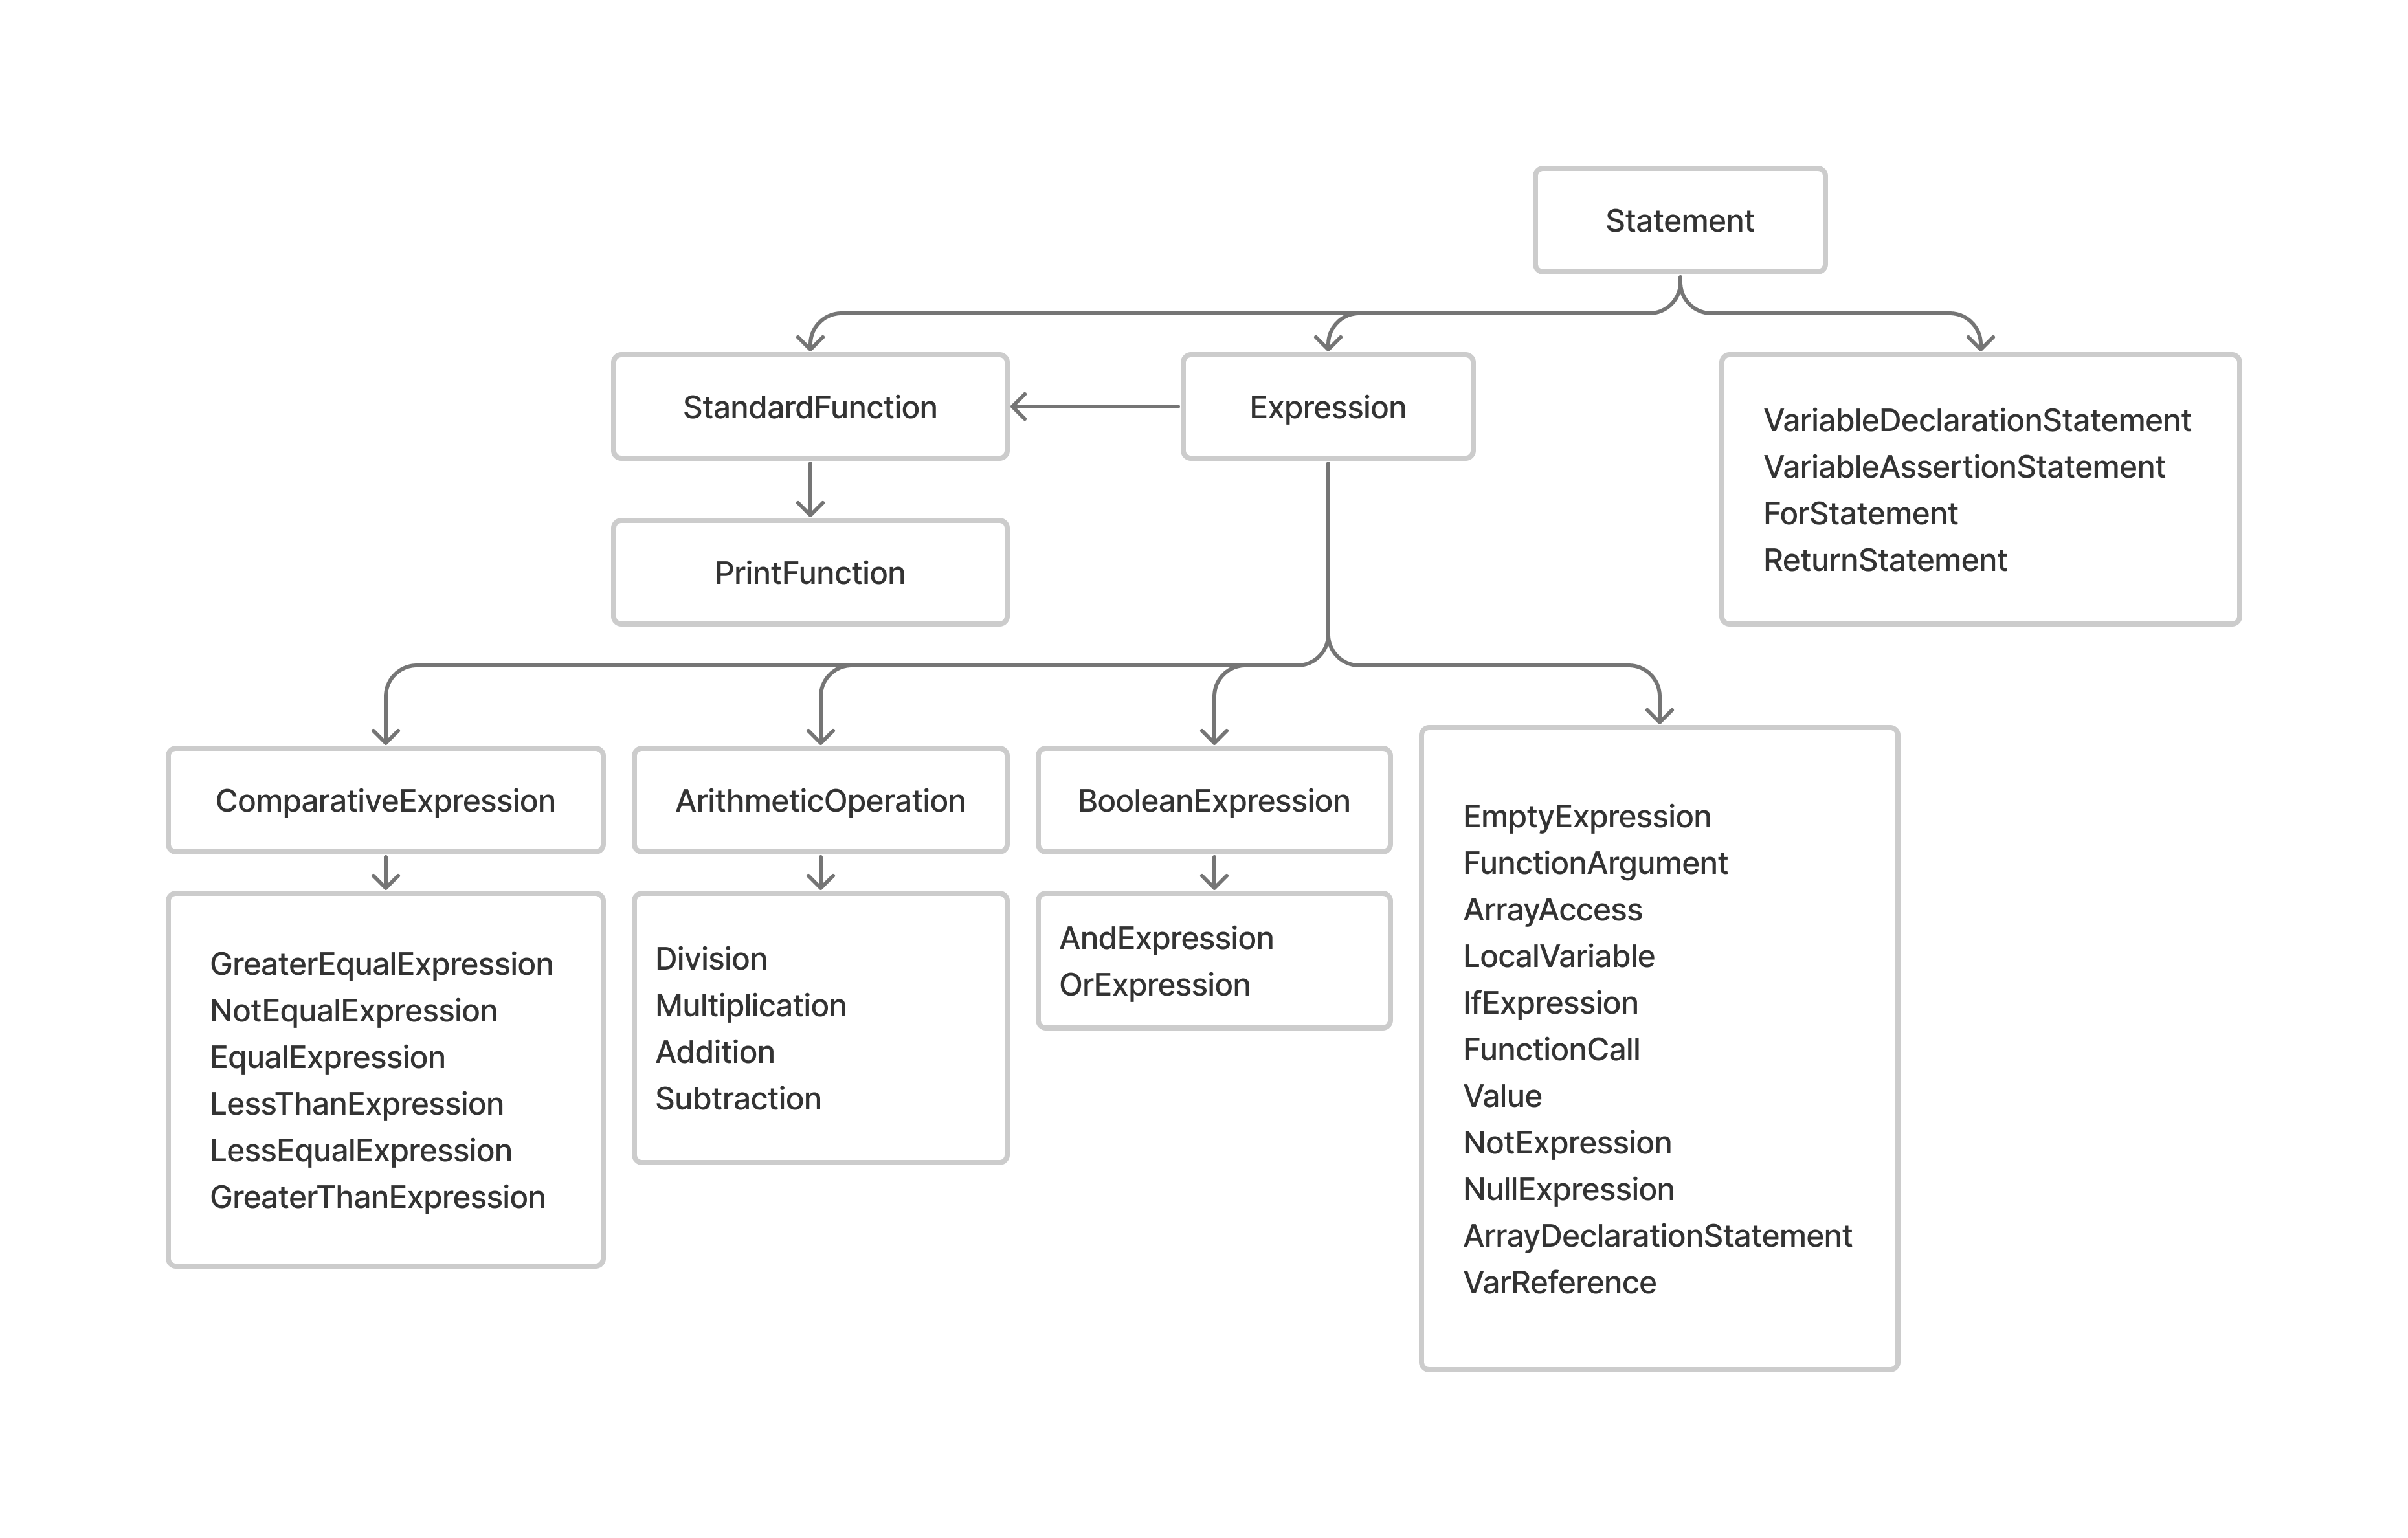
\includegraphics[scale=0.2]{AST.Diagram}
    \label{fig:ast-architecture}
\end{figure}

Kotlin bietet zur kompakten Erstellung von Datenobjekten sogenannte \textit{data classes} an. \texttt{data class} Objekte erzeugen für Mitglieder des primären Konstruktor folgende Funktionen:

\begin{itemize}
    \item \texttt{equals()} und \texttt{hashCode()}.
    \item \texttt{toString()} im Format \texttt{Addition(left=42, right=31)}.
    \item \texttt{componentN()}, die bei der Destrukturierung von Objekten verwendet werden. Hierbei ist die Reihenfolge der Definition relevant.
    \item \texttt{copy()} zum durchführen einer tiefen Kopie des Objekte.
\end{itemize}

\Toya verwendet \textit{data classes} für fast alle Klassen des AST. Ausgenommen sind Basisklassen, von denenen andere Klassen ableiten, da die Vererbung von \textit{data classes} zu Problemen mit dem Verhalten von \textit{equals()} zum Beispiel führt. Java bietet seit Version 14 \texttt{record} als Äquivalent zu diesem Konzept an. Jedoch fehlen bei \texttt{record} die \texttt{copmonentN()} und \texttt{copy()} Funktionen.

Die \texttt{Scope} Klasse ist eine zentrale Komponente in der Verwaltung des AST und wird unter anderem für die semantische Analyse benötigt. Sie speichert die lokalen Variablen für einen gegebenen Block und die Methodensignaturen eines \toya Programms. Bei Operationen, deren Operanden lokale Variablen sind, überprüft \toya mithilfe von \texttt{Scope}, ob diese Variablen im momentanten Kontext zur Verfügung stehen.

Im Zuge der Bytecode-Generierung ermittelt \toya mithilfe \scope den Index einer lokalen Variable. Hierbei reicht es nicht aus, den Index der Variable in der Liste \texttt{localVariables} zu ermitteln. Variablen vom Typ \texttt{double} und \texttt{long} benötigen zwei Plätze im \textit{Run-Time Constant Pool}, da deren Indizes 16 Bit, anstatt der üblichen acht Bit einnehmen. Da \toya den Typ Double implementiert, ist diese Eigenschaft zu berücksichtigen. Diese Berechnung erfolgt durch eine Reduktions-Operation in der Funktion \texttt{getLocalVariableIndex}, wie in~\autoref{lst:impl_localvariable} zu sehen ist. Diese Reduktions-Operation summiert alle Indizes bis inklusive dem Index der gesuchten Variable auf und addiert pro Index eins, beziehungsweise zwei, wenn die Variable vom Typ \texttt{double} ist.

\begin{KotlinCode}[numbers=none, caption={Ermittlung des Index einer Variable in einem \texttt{Scope}}, label=lst:impl_localvariable]
fun getLocalVariableIndex(varName: String) : Int {
    // hotfix for handling 2-wide index types (double, long, etc)
    return localVariables
        .subList(0, localVariables.indexOf(getLocalVariable(varName)))
        .fold(0) { acc, next ->
            acc + if (next.type == BasicType.DOUBLE) 2 else 1
        }
}
\end{KotlinCode}

\texttt{Scope} verwaltet nicht nur Variablen, sondern auch Funktionssignaturen. Beim Aufruf einer Funktion, überprüft \scope, ob diese Funktion auch definiert ist. Wenn nicht, tritt der Ausnahmezustand \texttt{MethodSignatureNotFoundException} ein. Während das Überladen von Funktionen erlaubt ist, können keine Funktionen mit identischer Signatur existieren, da diese in einem \texttt{Set} gespeichert sind.

\section{Backend}

Das Backend hat als zentrale Aufgabe die Code-Generierung anhand des abstrakten Syntaxbaums, den das Frontend erzeugt hat. Zum Erzeugen des Bytecodes verwendet das Backend ObjectWeb ASM als zentrale Bibliothek. Als Resultat liefert das Backend ein Byte-Feld, das anschließend ein \texttt{FileOutputStream} in eine class-Datei schreibt.

\subsection{ObjectWeb ASM}

ObjectWeb ASM ist eine Bibliothek zum Lesen, Bearbeiten und Erzeugen von Bytecode für die JVM. Sie bietet eine Schnittstelle, um Funktionen, Klassen und einzelne Anweisungen zu erzeugen. \Toya verwendet ASM zum Erzeugen einer Klasse und Funktionen anhand des AST. Neben der Bytecode-Generierung erfolgt im Backend der Teil der semantischen Analyse für welchen Informationen des AST notwendig sind. ASM ist kein Akronym sondern eine Anlehnung an das Schlüsselwort \texttt{asm} in der Programmiersprache C \parencite{bruneton2002asm}.

Da \toya keine Definition von Klassen erlaubt, reicht es aus, eine statische Klasse, unabhängig vom eigentlichen Quelltext zu generieren. Version dieser Klasse ist 52, was Java 8 entspricht. Einen höhere Version ist nicht nötig, da alle Bestandteile von \toya sehr primitiv sind.

Klassen erstellt ASM mithilfe des \texttt{ClassWriter}. Der Konstruktor dieser Klasse hat einen Parameter \texttt{flags}. Im Falle von \toya ist dies \texttt{COMPUTE\_FRAMES + COMPUTE\_MAXS}. \texttt{COMPUTE\_MAXS} und \texttt{COMPUTE\_FRAMES} ermöglicht die automatische Berechnung der maximal erlaubten Anzahl an lokalen Variablen, die maximale Größe des Stacks und die Berechnung aller \textit{Stack Map Frames}. Siehe dazu~\autoref{lst:impl_classwriter}.

\begin{KotlinCode}[numbers=none, caption={Erstellung einer Klasse mithilfe ObjectWeb ASM}, label=lst:impl_classwriter]
val classWriter: ClassWriter = ClassWriter(
    ClassWriter.COMPUTE_FRAMES + ClassWriter.COMPUTE_MAXS
)
classWriter.visit(
    CLASS_VERSION,
    Opcodes.ACC_PUBLIC,
    className,
    null,
    "java/lang/Object",
    null
)
\end{KotlinCode}

Zum Erzeugen von Methoden und und deren Logik bietet ObjectWeb ASM die Klasse \texttt{MethodWriter}. Diese Klasse ermöglicht das Schreiben der Bytecode Anweisungen innerhalb einer Methode. Außerdem ermöglicht \texttt{MethodWriter} unter anderem auch das Setzen von \textit{Labels} um Sprung-Befehle durchführen zu können. Sprung-Befehle sind für den Kontrollfluss wichtig, um in If-Verzweigungen nicht zutreffende Zweige zu überspringen und um bei For-Schleifen an den Beginn der Schleife zurückzukehren.~\autoref{lst:impl_generateexample} zeigt die \texttt{generate}-Funktion zum Generieren von Wertliteralen mithilfe von ObjectWeb ASM.

\begin{KotlinCode}[numbers=none, caption={\texttt{generate()} Funktion, welche Wert-Literale erzeugt.}, label=lst:impl_generateexample]
private fun generate(value: Value) {
    val type = value.type
    val stringValue = value.value

    type.handleTypeGroups(
        i = {
            val intValue = stringValue.toInt()
            methodVisitor.visitLdcInsn(intValue)
        },
        d = {
            val doubleValue = stringValue.toDouble()
            methodVisitor.visitLdcInsn(doubleValue)
        },
        a = { methodVisitor.visitLdcInsn(stringValue.trim('"')) },
        z = {
            val opcode = if (stringValue == "true") Opcodes.ICONST_1 else Opcodes.ICONST_0
            methodVisitor.visitInsn(opcode)
        }
    )
}
\end{KotlinCode}

\subsection{Summentypen}

Im Backend kommen Summentypen in Form von \textit{sealed classes} zum Einsatz. \textit{Sealed classes} in Kotlin besitzen die besondere Eigenschaft, dass alle Kindklassen zur Übersetzungszeit vollständig bekannt sind. Dies ermöglicht zum Beispiel die Verwendung von erschöpfenden \texttt{when}-Ausdrücken in Kombination mit Polymorphismus. Kindklassen einer \textit{sealed class} sind alle im selben Modul zu definieren. Neben Klassen können auch Schnittstellen als \texttt{sealed} markiert sein. Ist eine Klasse als \textit{sealed} markiert, ist diese Klasse zusätzlich implizit eine abstrakte Klasse.

Wichtige \textit{sealed classes} und \textit{sealed interfaces} des abstrakten Syntaxbaums sind folgende:

\begin{itemize}
    \item \texttt{ArithmeticOperation}: Umfasst Ausdrücke Addition, Subtraktion, Multiplikation und Division.
    \item \texttt{BooleanExpression}: Umfasst Ausdrücke für die logischen Operatoren \texttt{Und} und \texttt{Oder}. Eine \texttt{BooleanExpression} liefert immer einen boole'schen Wert zurück.
    \item \texttt{ComparativeExpression}: Umfasst Ausdrücke für Größer, Größer-Gleich, Gleich, Kleiner, Kleiner-Gleich und Ungleich. Eine \texttt{ComparativeExpression} liefert immer einen boole'schen Wert zurück.
    \item \texttt{Branch}: Umfasst die beiden Möglichkeiten, Verzweigungen im Kontrollfluss entweder als Anweisungsblock oder als einzelnen Ausdruck zu definieren.
\end{itemize}

\subsection{Architektur der Code-Generierung}

Der Ablauf der Code-Generierung ist auf fünf Klassen aufgeteilt, wie in~\autoref{fig:backend-flowchart} zu sehen ist. Als Einstiegspunkt dient immer die Klasse \texttt{ByteCodeGenerator}. Diese Klasse erzeugt eine öffentliche Klasse, die von \texttt{Object} erbt. Als nächstes ruft \texttt{ByteCodeGenerator} für jede Funktion die \texttt{generate}-Methode des \texttt{FunctionGenerator} auf.

Der \texttt{FunctionGenerator} iteriert über die Liste aller Anweisungen der Funktion und ruft für jede Anweisung die \texttt{generate}-Funktion des \texttt{StatementGenerator auf}. Nach dem durchlaufen der Anweisungsliste überprüft der \texttt{FunctionGenerator}, ob die Funktion als letzte Anweisung eine Rückgabeanweisung definiert und ob die Funktion überhaupt einen Wert zurückliefert. Liefert nun die Funktion einen Wert zurück, hat aber keine Rückgabeanweisung an letzter Stelle, ist diese Anweisung zu generieren. Anhand des Typs der letzten Anweisung der Funktion wählt der \texttt{FunctionGenerator} nun den richtigen Opcode aus und generiert die Anweisung mithilfe von ObjectWeb ASM. Ist die letzte Anweisung zum Beispiel eine Ganzzahl, generiert der \toya-Compiler den Opcode \texttt{ireturn}.

Der \texttt{StatementGenerator} generiert entweder eine Anweisung selbst oder delegiert diese Aufgabe an den \texttt{ExpressionGenerator}, wenn es sich bei der Anweisung um einen Ausdruck handelt. Konkret generiert der \texttt{StatementGenerator} Bytecode für Variablen- und Felddeklarationen, Variablenzuweisungen, explizite Rückgabeanweisungen und For-Schleifen. Ein Großteil der Komplexität in dieser Klasse stammt daher, dass verschiedene Opcode für die verschiedenen Typen von \toya zu beachten sind.

\begin{figure}[h]
    \caption{Ablauf der Code-Generierung im Backend.}
    \centering
    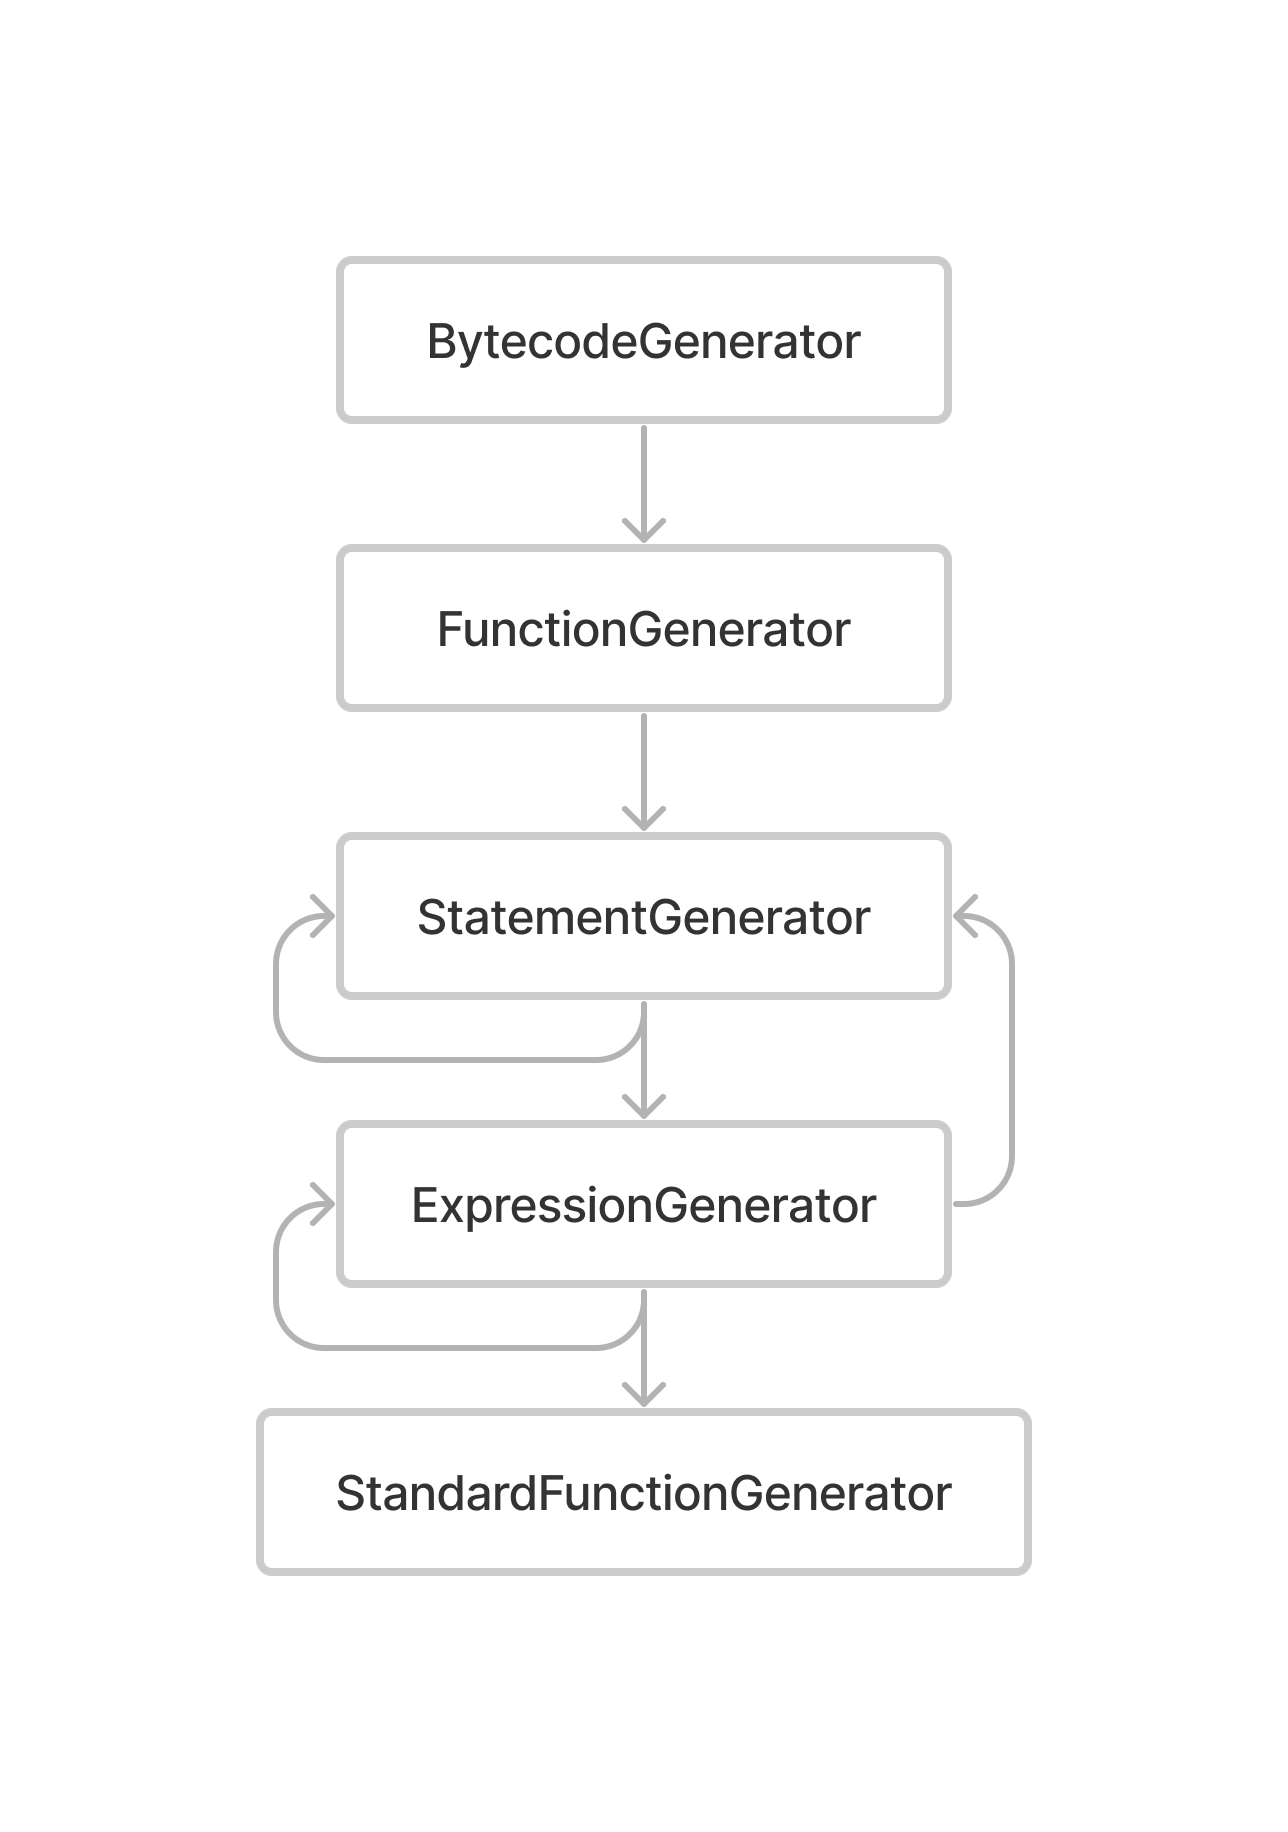
\includegraphics[scale=0.3]{Backend.Flowchart}
    \label{fig:backend-flowchart}
\end{figure}

Um den Mehraufwand für die Berücksichtigung jedes Typs so gut wie möglich zu minimieren, sind die Erweiterungsfunktionen \texttt{Type.handleTypeGroup()} und\break \texttt{Type.handleTypeArrays()} definiert, die Implementierung und Verwendung von letzteres ist in~\autoref{lst:impl_handletypearrays} zu sehen. Diese beiden Funktionen höherer Ordnung benötigen eine Funktion für jeden Typ als Parameter. Dadurch liegt in jeder Funktion nur der Code, der für den entsprechenden Typ relevant ist.

Ebenso ist auch die Ausnahmebehandlung mithilfe dieser Funktionen umsetzbar. Versucht man zum Beispiel zwei Referenzen oder boole'sche Ausdrücke zu addieren, tritt der Ausnahmezustand \texttt{UnsupportedOperationOnTypeException} ein. Dadurch, dass das Verhalten für jeden Typ verpflichtend definiert sein muss, vermeidet die Entwickler:in auch, dass das Verhalten für einen Typ ungeklärt bleibt.

\begin{KotlinCode}[numbers=none, caption={Die Erweiterungsfunktion \texttt{Type.handleTypeArrays()}, um den richtigen Opcode zum Speichern einer Variable zu ermitteln.}, label=lst:impl_handletypearrays]
fun <T> Type.handleTypeArrays(
    ia: () -> T,
    da: () -> T,
    aa: () -> T,
    ba: () -> T
): T {
    return when (this) {
        BasicType.INT_ARR -> ia()
        BasicType.DOUBLE_ARR -> da()
        BasicType.STRING_ARR -> aa()
        BasicType.BOOLEAN_ARR -> ba()
        else -> throw NotImplementedError("handling for type '\${this.typeName}' not implemented")
    }
}

val opcode = localVariable.type.handleTypeArrays(
    ia = { Opcodes.IASTORE },
    da = { Opcodes.DASTORE },
    aa = { Opcodes.AASTORE },
    ba = { Opcodes.BASTORE }
)
\end{KotlinCode}

Der \texttt{ExpressionGenerator} generiert Ausdrücke oder delegiert Standardfunktionsaufrufe an den \texttt{StandardFunctionGenerator}. Ist der konkrete Typ des Ausdrucks \texttt{PrintFunction}, delegiert der \texttt{ExpressionGenerator} die Bytecode-Generierung an den \texttt{StandardFunctionGenerator}. Konkret generiert der \texttt{ExpressionGenerator} Bytecode für folgende Ausdrücke:

\begin{itemize}
    \item Variablenaufrufe
    \item Funktionsaufrufe
    \item Funktionsargumente
    \item Wertliterale
    \item arithmetische Operationen
    \item Vergleichsoperationen
    \item Logikoperationen
    \item Null-Ausdrücke
    \item Zugriff auf Felder
    \item If-Ausdrücke
\end{itemize}

Der \texttt{StandardFunctionGenerator} generiert alle Standardfunktionen. Im Falle der \texttt{PrintFunction} verwendet \toya die \texttt{System.out.println} Implementierung von Java. In einem ersten Schritt ermittelt \toya die Referenz des \texttt{PrintSteam} Typs in Form der statischen Variable \texttt{out} und evaluiert \toya den Wert des Ausdrucks, der auszugeben ist. Anschließend wird die \texttt{println} Funktion des \texttt{out} Objekts aufgerufen. Die \texttt{println} Funktion verwendet den oben aufliegenden Wert am Operanden-Stack, weswegen dieser Wert im ersten Schritt bereits evaluiert wurde. Die konkrete Implementierung, wie in~\autoref{lst:impl_println} zu sehen ist, wurde \textcite{enkelTutorial} entnommen.

\begin{KotlinCode}[numbers=none, caption={Bytecode zum Aufruf der \texttt{println} Funktion von Java}]
private fun generate(printFunction: PrintFunction, scope: Scope) {
    val expression = printFunction.message
    mv.visitFieldInsn(Opcodes.GETSTATIC, "java/lang/System", "out", "Ljava/io/PrintStream;")
    expressionGenerator.generate(expression, scope)
    val type = expression.type
    val descriptor = "(\${type.getDescriptor()})V"
    val fieldDescriptor = "java/io/PrintStream"
    mv.visitMethodInsn(Opcodes.INVOKEVIRTUAL, fieldDescriptor, "println", descriptor, false)
}
\end{KotlinCode}